\documentclass[letterpaper,12pt]{article}
\usepackage[spanish]{babel}
\usepackage[utf8]{inputenc}
\usepackage{graphicx}
\usepackage{geometry}
\usepackage{titlesec}
\usepackage{fancyhdr}
\usepackage{tcolorbox}
\usepackage{array}
\usepackage{tabularx}
\usepackage{hyperref}
\usepackage{float}
\usepackage{enumitem}
\usepackage{listings}
\usepackage{xcolor}

% ==================== CONFIGURACIÓN DE PÁGINA ====================
\geometry{top=3.5cm, bottom=3cm, left=2.5cm, right=2.5cm, headheight=2cm, footskip=2cm}

% ==================== FORMATO DE TÍTULOS ====================
\titleformat{\section}{\large\bfseries}{\thesection.}{0.6em}{}
\titleformat{\subsection}{\normalsize\bfseries}{\thesubsection}{0.6em}{}
\titleformat{\subsubsection}{\normalsize\bfseries\itshape}{\thesubsubsection}{0.6em}{}

% ==================== ENCABEZADO Y PIE ====================
\pagestyle{fancy}
\fancyhf{}
\fancyfoot[C]{\thepage}
\renewcommand{\headrulewidth}{0.4pt}
\rhead{\textit{Material de Ayuda}}
\lhead{\textit{Tarea ELO323 / IPD438}}

% ==================== HIPERVÍNCULOS ====================
\hypersetup{
    colorlinks=true,
    linkcolor=blue,
    urlcolor=blue,
    citecolor=blue
}

% ==================== ESTILO PARA CÓDIGO / COMANDOS ====================
\definecolor{codegray}{gray}{0.95}
\definecolor{codekeyword}{rgb}{0.0,0.0,0.6}
\lstset{
    basicstyle=\ttfamily\small,
    backgroundcolor=\color{codegray},
    frame=single,
    breaklines=true,
    columns=fullflexible,
    keepspaces=true,
    xleftmargin=0.4cm,
    xrightmargin=0.4cm,
    aboveskip=8pt,
    belowskip=8pt
}

% ==================== CAJAS DE COLOR ====================
% Caja para notas generales
\newtcolorbox{nota}{colback=yellow!8!white, colframe=orange!70!black, title=Nota, fonttitle=\bfseries}
% Caja para actividades reservadas a la investigación del estudiante
\newtcolorbox{investigar}{colback=blue!5!white, colframe=blue!55!black, title=Reservado para investigación del estudiante, fonttitle=\bfseries}

% ==================== MACRO PARA PLACEHOLDER DE FIGURAS ====================
% Uso: \figplaceholder{descripcion del contenido}{texto del caption}
\newcommand{\figplaceholder}[2]{%
    \begin{figure}[H]
        \centering
        \fbox{\begin{minipage}[c][4.2cm][c]{0.8\textwidth}
            \centering \textit{[ Espacio reservado para captura ]}\\[0.3cm]
            \small #1
        \end{minipage}}
        \caption{#2}
    \end{figure}%
}

\begin{document}

% ==================== PORTADA ====================
\thispagestyle{empty}

\begin{center}
    % Logo institucional (carpeta 'images'); el trim recorta el margen blanco del PNG
    
\includegraphics[width=0.9\textwidth, trim=134 278 134 278, clip]{images/INS_h_color@2x.png} \\[2.5cm]
    {\LARGE \textbf{Material de Ayuda}}\\[0.5cm]
    {\large Tarea ELO323 / IPD438 -- ``Emulando Redes con GNS3''}\\[0.5cm]
    {\large Redes de Computadores II}\\[0.3cm]
    {\large Seminario de Redes de Computadores}\\[2.4cm]

    \hspace{3cm}\begin{tabular}{|l|l|}
        \hline
        Asignatura:  & ELO323 / IPD438 \\ \hline
        Semestre:    & 2\textordmasculine{} Semestre 2026 \\ \hline
        Última actualización: & 2026 \\ \hline
    \end{tabular}
\end{center}

\vfill
\begin{center}
    \small \textit{Revisión 2\textordmasculine{} Semestre 2026 por Nicolás Rogel}
\end{center}

\newpage

% ==================== ÍNDICE ====================
\tableofcontents
\newpage

% ==================== GNS3 ====================
\section{GNS3}

GNS3 es un \textbf{software emulador de redes} (revisar diferencia entre \href{https://en.wikipedia.org/wiki/Network_simulation}{simulador de redes} y \href{https://en.wikipedia.org/wiki/Network_emulation}{emulador de redes}). Este programa trabaja principalmente con máquinas virtuales, permitiendo la \textbf{emulación de equipos reales}, como switches y routers. Si bien es un emulador de redes, su sigla corresponde a ``Graphical Network Simulator-3'', por esto en este material se usará el término simulador para referirse a él. Es posible además conectar las redes simuladas con dispositivos externos.

\subsection{Instalación en Windows}

El software de GNS3 se distribuye en la \href{https://www.gns3.com/}{página web de GNS3}. Basta con descargar la versión disponible para \href{https://www.gns3.com/software/download}{Windows} (la página previamente pedirá crear una cuenta), y seguir la \textbf{configuración por defecto del instalador}. En la pantalla \textit{Choose Components} el instalador ofrece varios programas adicionales; no todos son necesarios para esta tarea, y omitir los innecesarios deja una instalación más liviana:

\begin{itemize}
    \item \textbf{Dejar marcados:} \textbf{GNS3} (siempre requerido), \textbf{WinPCAP} o \textbf{Npcap} (requerido por el nodo Nube para comunicarse con la red exterior, Pregunta 3), \textbf{Wireshark} (captura de paquetes en los enlaces), \textbf{Dynamips} (ejecuta el router Cisco 3725), \textbf{VPCS} (terminales de la Pregunta 1) y \textbf{Solar-PuTTY} (consola por defecto para acceder a los equipos).
    \item \textbf{Se pueden desmarcar:} \textbf{QEMU} (las máquinas QEMU de la tarea se ejecutan dentro de la GNS3 VM), \textbf{TightVNC Viewer} y \textbf{Virt-viewer} (solo sirven para máquinas con interfaz gráfica; la máquina Alpine no tiene), \textbf{Cpulimit} (solo necesario con equipos antiguos como el ASA) e \textbf{Intel HAXM}.
\end{itemize}

Al concluir la instalación, \textbf{no iniciar el programa hasta terminar los pasos descritos a continuación}.

\begin{nota}
Este material fue verificado con \textbf{GNS3 2.2.61} (Windows y Linux) y \textbf{VirtualBox 7.2.16}. Se recomienda usar estas versiones o superiores compatibles.
\end{nota}

Para obtener un \textbf{desempeño razonable} de las máquinas virtuales en Windows, se recomienda utilizar la máquina virtual ofrecida por GNS3, que puede descargarse desde \href{https://gns3.com/software/download-vm}{GNS3 VM}. Es importante que sea de la \textbf{misma versión que la aplicación de GNS3}. Al descomprimir este archivo se obtiene un archivo con extensión \texttt{.ova} que se usará más adelante.

Para continuar con la configuración de la máquina virtual, es necesario descargar e instalar el software \href{https://www.virtualbox.org/wiki/Downloads}{VirtualBox} de Oracle (VirtualBox 7.2.16). Seguir la configuración por defecto del instalador.

\begin{nota}
Los desarrolladores de GNS3 recomiendan un hipervisor con virtualización anidada (nested virtualization) para mejor rendimiento. En muchos equipos con VirtualBox sobre Windows, la virtualización anidada (KVM\footnotemark) \textbf{no está disponible}. Esto se aborda en la sección \textit{Ejecución sin KVM}. Sugerencia: en lo posible, considere utilizar Linux para correr GNS3.
\end{nota}
\footnotetext{KVM (\textit{Kernel-based Virtual Machine}) es una tecnología de virtualización integrada en el kernel de Linux, que permite a una máquina física actuar como múltiples entornos virtuales aislados, compartiendo el hardware de forma directa y eficiente.}

Concluida la instalación, ejecute VirtualBox, seleccione \textbf{``Archivo $>$ Importar servicio virtualizado''} e importe el archivo \texttt{GNS3 VM.ova} descargado previamente con las características por defecto. De esta forma queda cargada la máquina virtual de GNS3 VM. Concluido este paso, continúe con la \textbf{Inicialización}.

\subsection{Instalación en Linux (Ubuntu)}

Para distribuciones basadas en Ubuntu, basta con agregar el repositorio de GNS3 a \texttt{apt} y luego instalarlo:

\begin{lstlisting}
sudo add-apt-repository ppa:gns3/ppa
sudo apt update
sudo apt install gns3-server gns3-gui
sudo dpkg --add-architecture i386
sudo apt update
sudo apt install gns3-iou
\end{lstlisting}

\begin{nota}
Durante la instalación se consulta por configuraciones específicas; se sugiere aceptar las opciones por defecto.
\end{nota}

En caso de requerir una \textbf{guía en video}, se recomienda el tutorial \href{https://www.youtube.com/watch?v=PBdHzJOi1Tc}{Tutorial GNS3 Ubuntu}. Para otras distribuciones, el procedimiento es similar cambiando el gestor de paquetes; ver las \href{https://docs.gns3.com/docs/getting-started/installation/linux/}{instrucciones oficiales de GNS3}.

Para el caso de Linux, a diferencia de Windows, \textbf{no es necesario instalar la máquina virtual de GNS3 ni el virtualizador VirtualBox}, debido a que lo solicitado en la tarea es lo suficientemente estable en Linux.

\subsection{Inicialización}

La primera vez que se abre GNS3 se presenta automáticamente el \textbf{asistente de inicialización} (\textit{Setup Wizard}). Si no aparece, o si necesita volver a ejecutarlo más adelante (por ejemplo, para cambiar de servidor), ábralo desde el menú \textbf{Help} de la barra de menús superior (1), opción \textbf{Setup Wizard} (2), como muestra la Figura~\ref{fig:help}.

\begin{figure}[H]
    \centering
    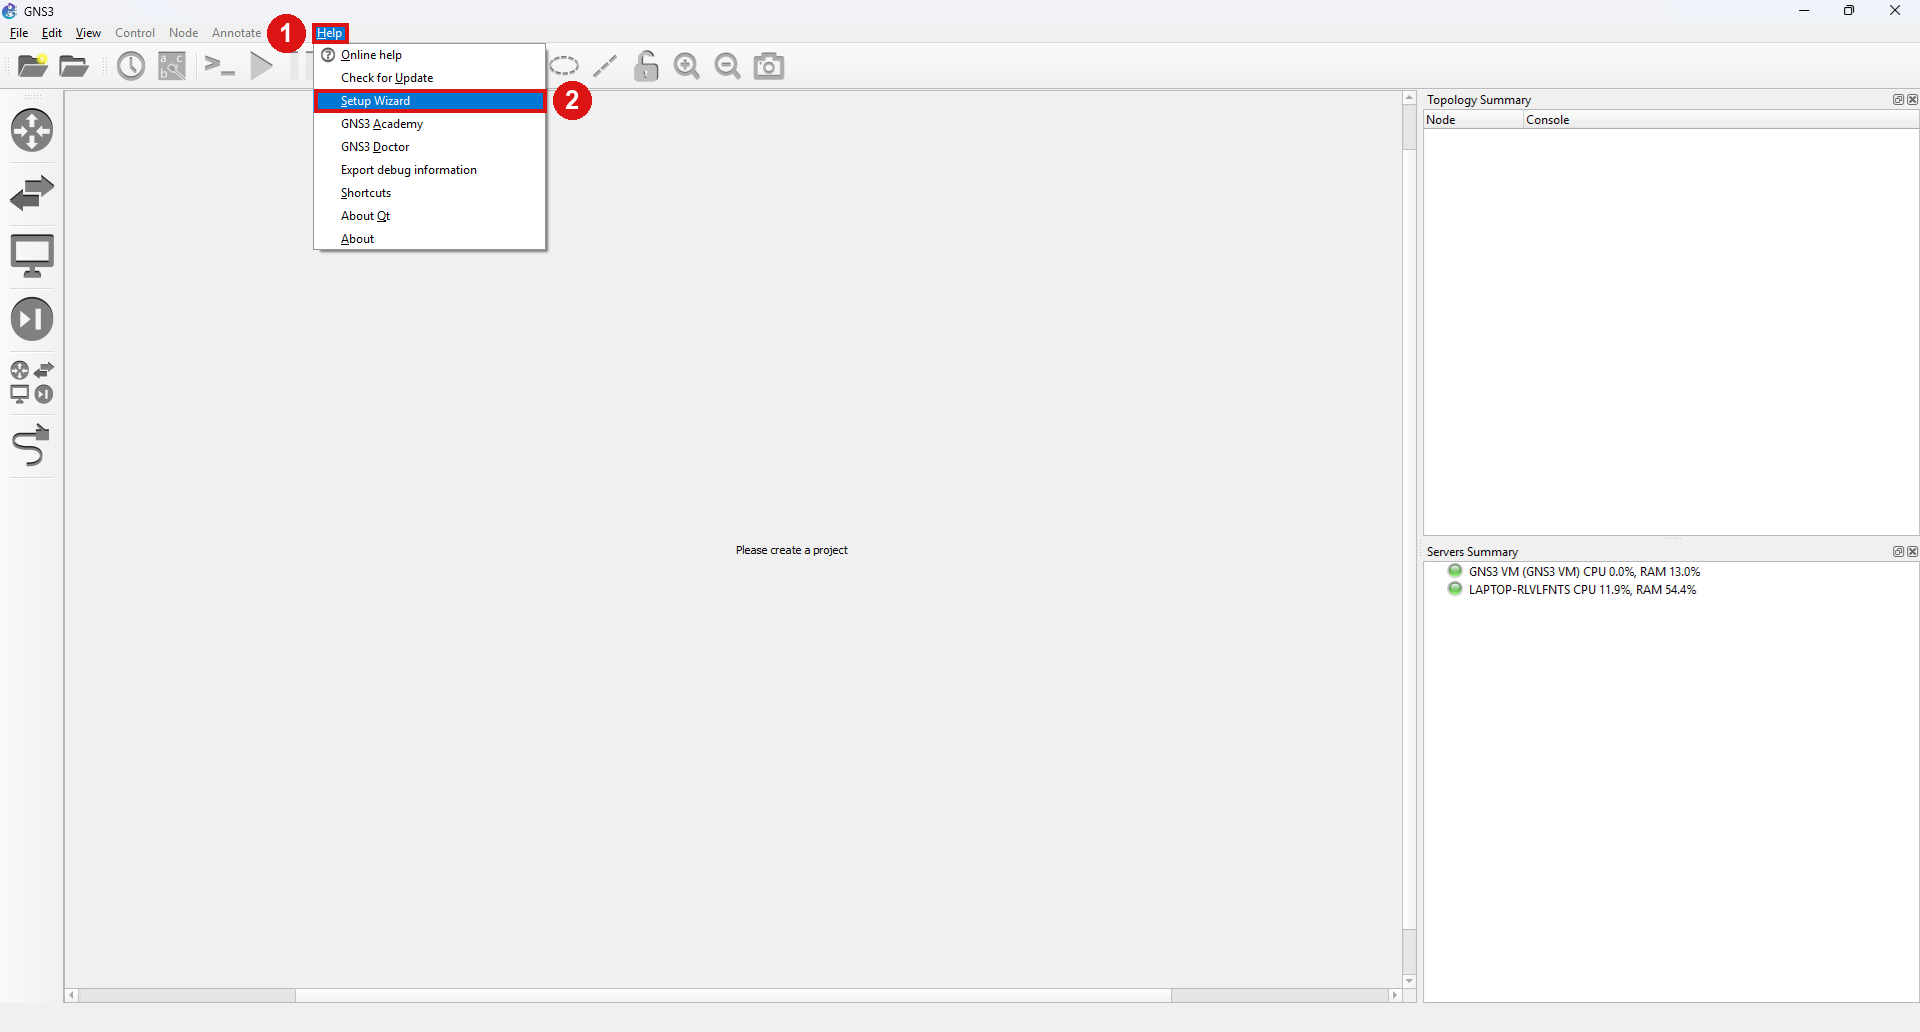
\includegraphics[width=\textwidth]{images/gns3_help_setup_wizard.png}
    \caption{Acceso al asistente de inicialización: menú \textit{Help} (1) $>$ \textit{Setup Wizard} (2).}
    \label{fig:help}
\end{figure}

El primer paso del asistente es escoger \textbf{dónde se ejecutarán los equipos simulados} (Figura~\ref{fig:wiz-servidor}). En Windows, seleccione \textit{Run appliances in a virtual machine} (1), que utiliza la GNS3 VM importada en VirtualBox, y presione \textit{Next} (2). En Linux, donde no se usa la GNS3 VM, seleccione en cambio \textit{Run appliances on my local computer}.

\begin{figure}[H]
    \centering
    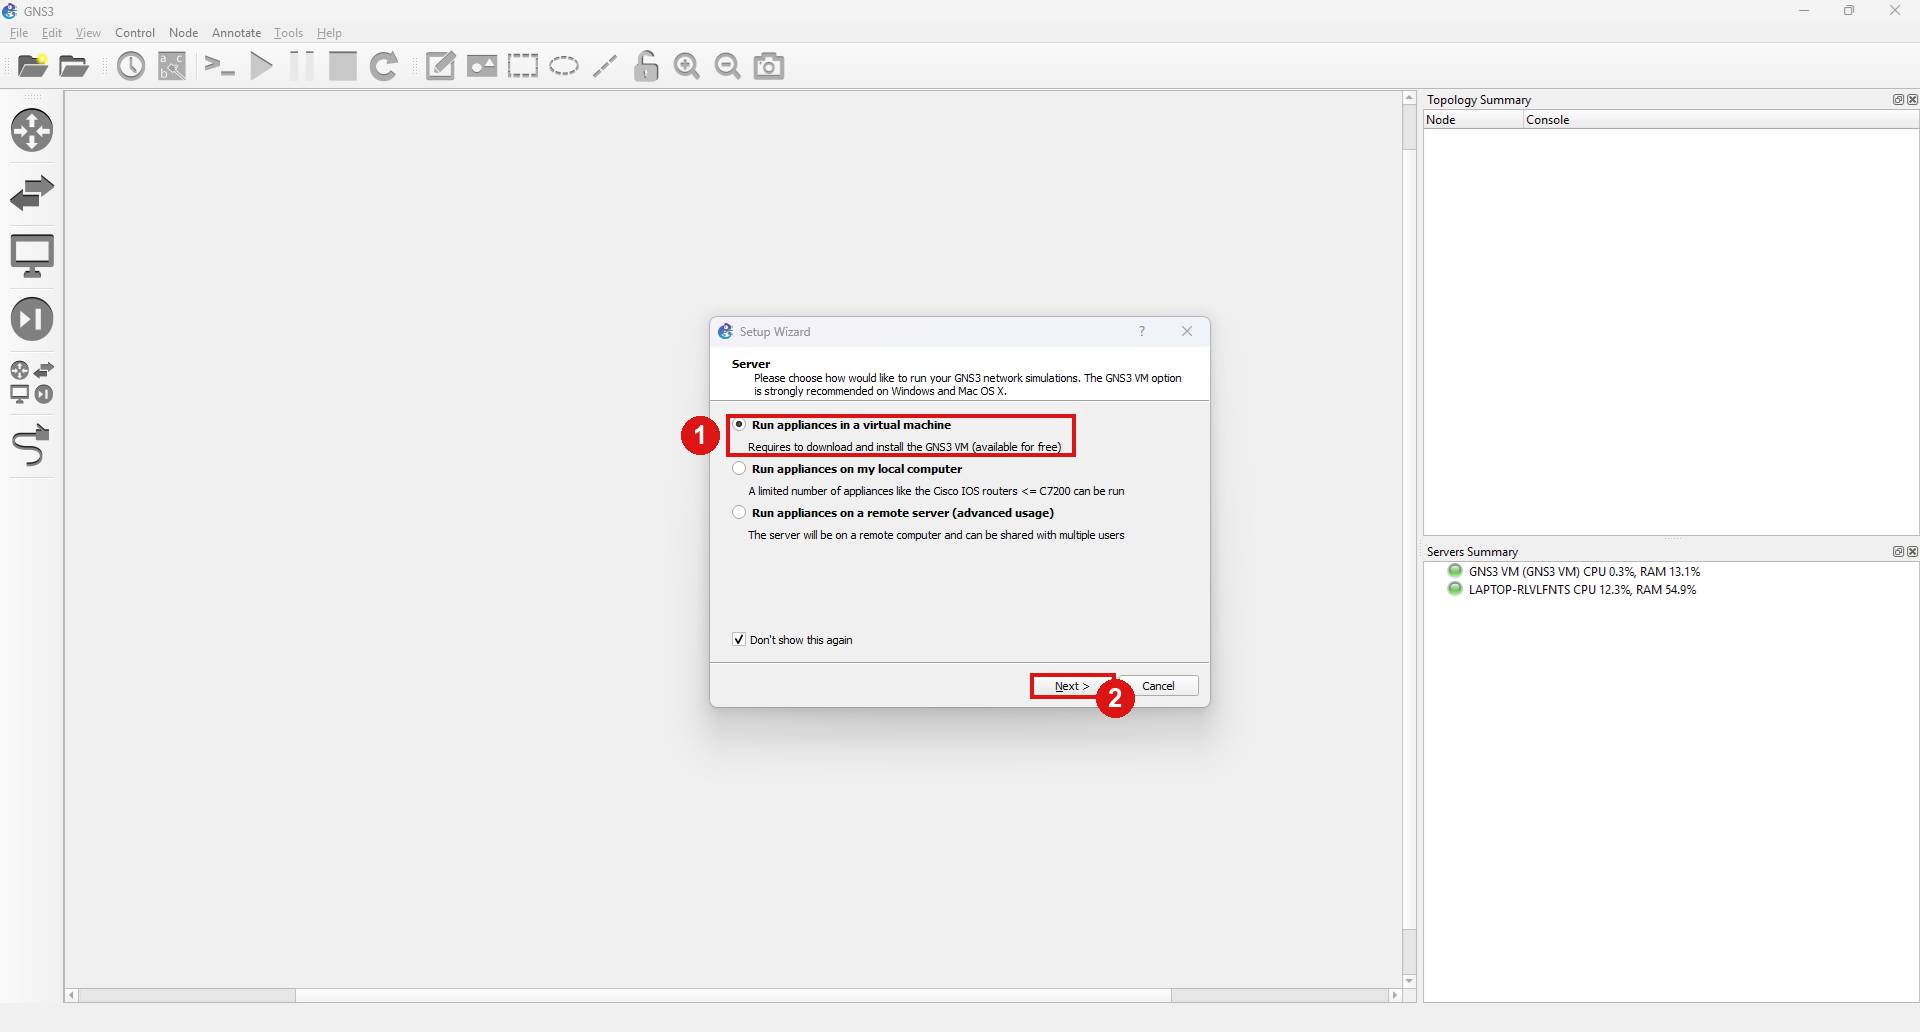
\includegraphics[width=\textwidth]{images/gns3_wizard_tipo_servidor.png}
    \caption{Asistente, paso 1: ejecutar los equipos en la GNS3 VM (1) y continuar (2).}
    \label{fig:wiz-servidor}
\end{figure}

A continuación se configura la GNS3 VM (Figura~\ref{fig:wiz-vm}). Seleccione \textbf{VirtualBox} como software de virtualización (1). Si la GNS3 VM fue importada correctamente, aparecerá en el campo \textit{VM name} (2); si no aparece, presione \textit{Refresh}. En los campos \textit{vCPU cores} y \textit{RAM size} se indican los recursos del computador que se asignan a la GNS3 VM; los valores por defecto (2 núcleos y 4096 MB) son suficientes para la tarea. Presione \textit{Next} (3).

\begin{figure}[H]
    \centering
    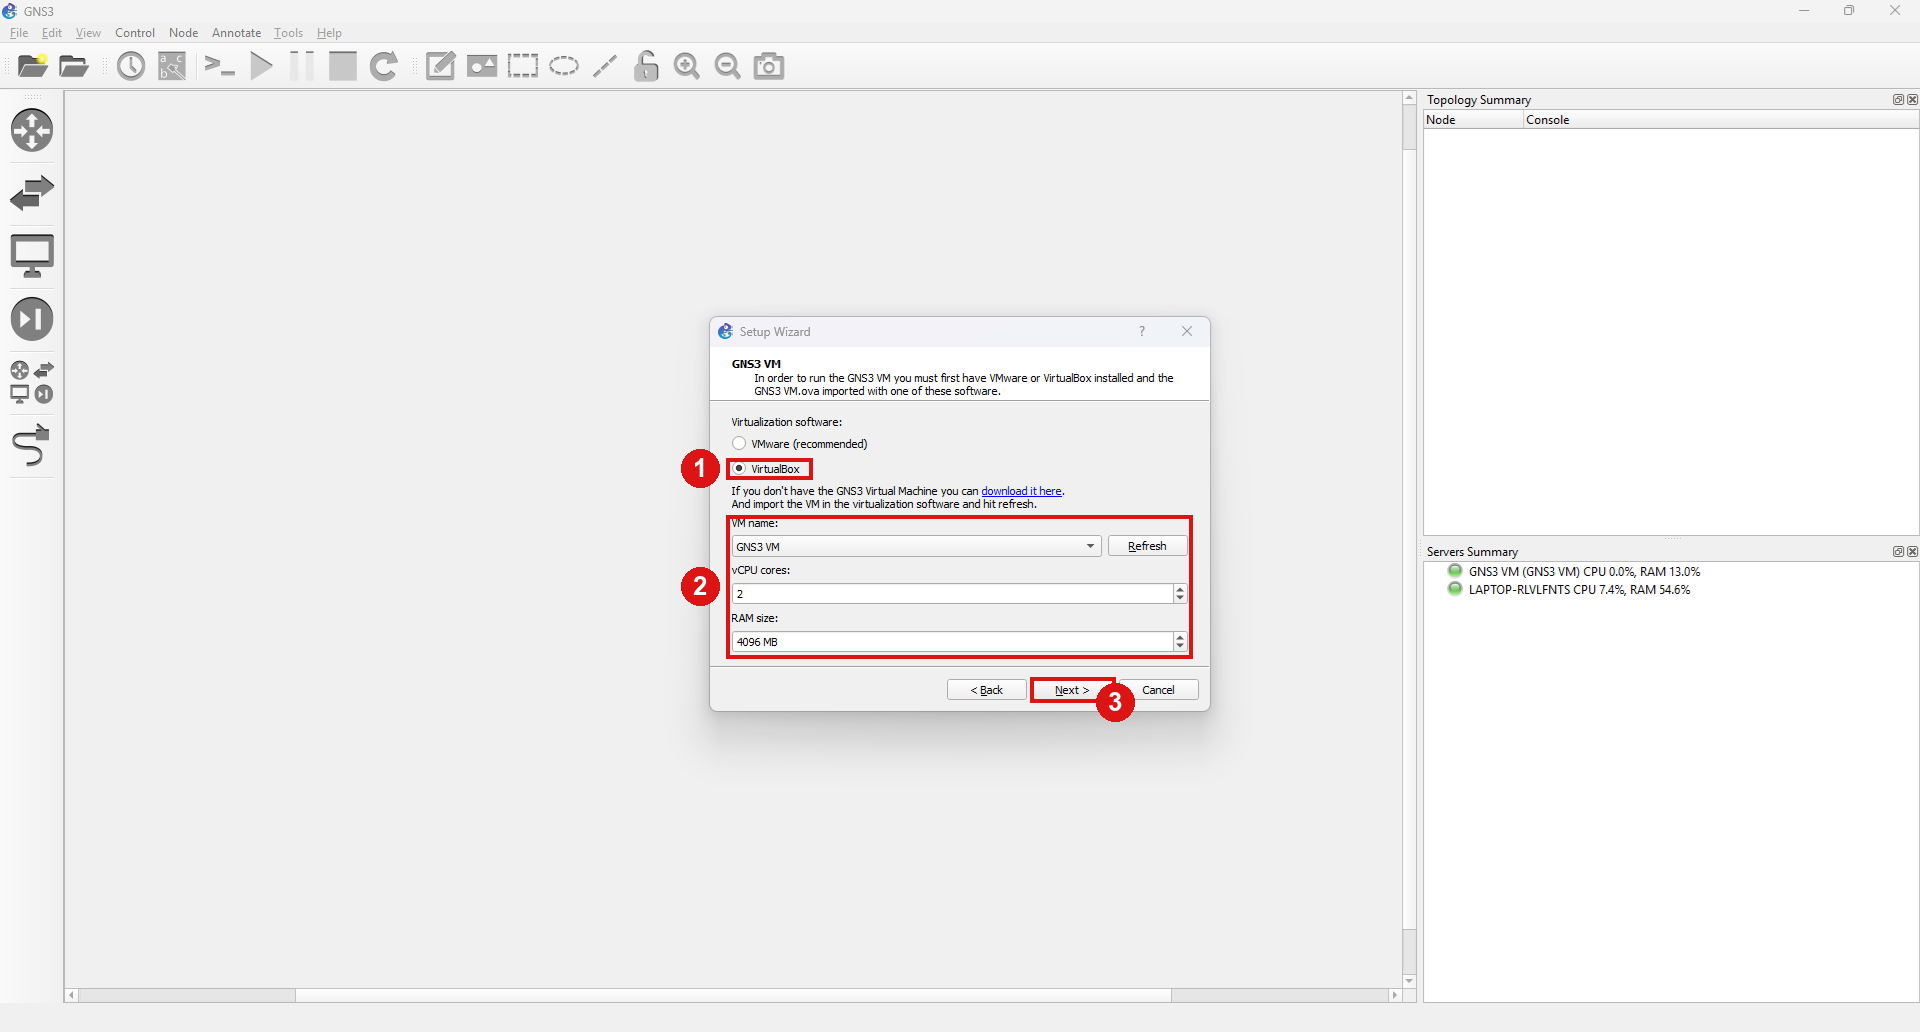
\includegraphics[width=\textwidth]{images/gns3_wizard_gns3vm.png}
    \caption{Asistente, paso 2: VirtualBox (1), selección y recursos de la GNS3 VM (2) y continuar (3).}
    \label{fig:wiz-vm}
\end{figure}

Finalmente, el asistente muestra un resumen de la configuración (1). Verifique que el tipo de servidor sea \textit{GNS3 Virtual Machine} con motor \textit{Virtualbox} y presione \textit{Finish} (2) (Figura~\ref{fig:wiz-resumen}). En el panel \textit{Servers Summary}, a la derecha de la ventana principal, la GNS3 VM debe aparecer con un círculo verde, lo que indica que está encendida y conectada.

\begin{figure}[H]
    \centering
    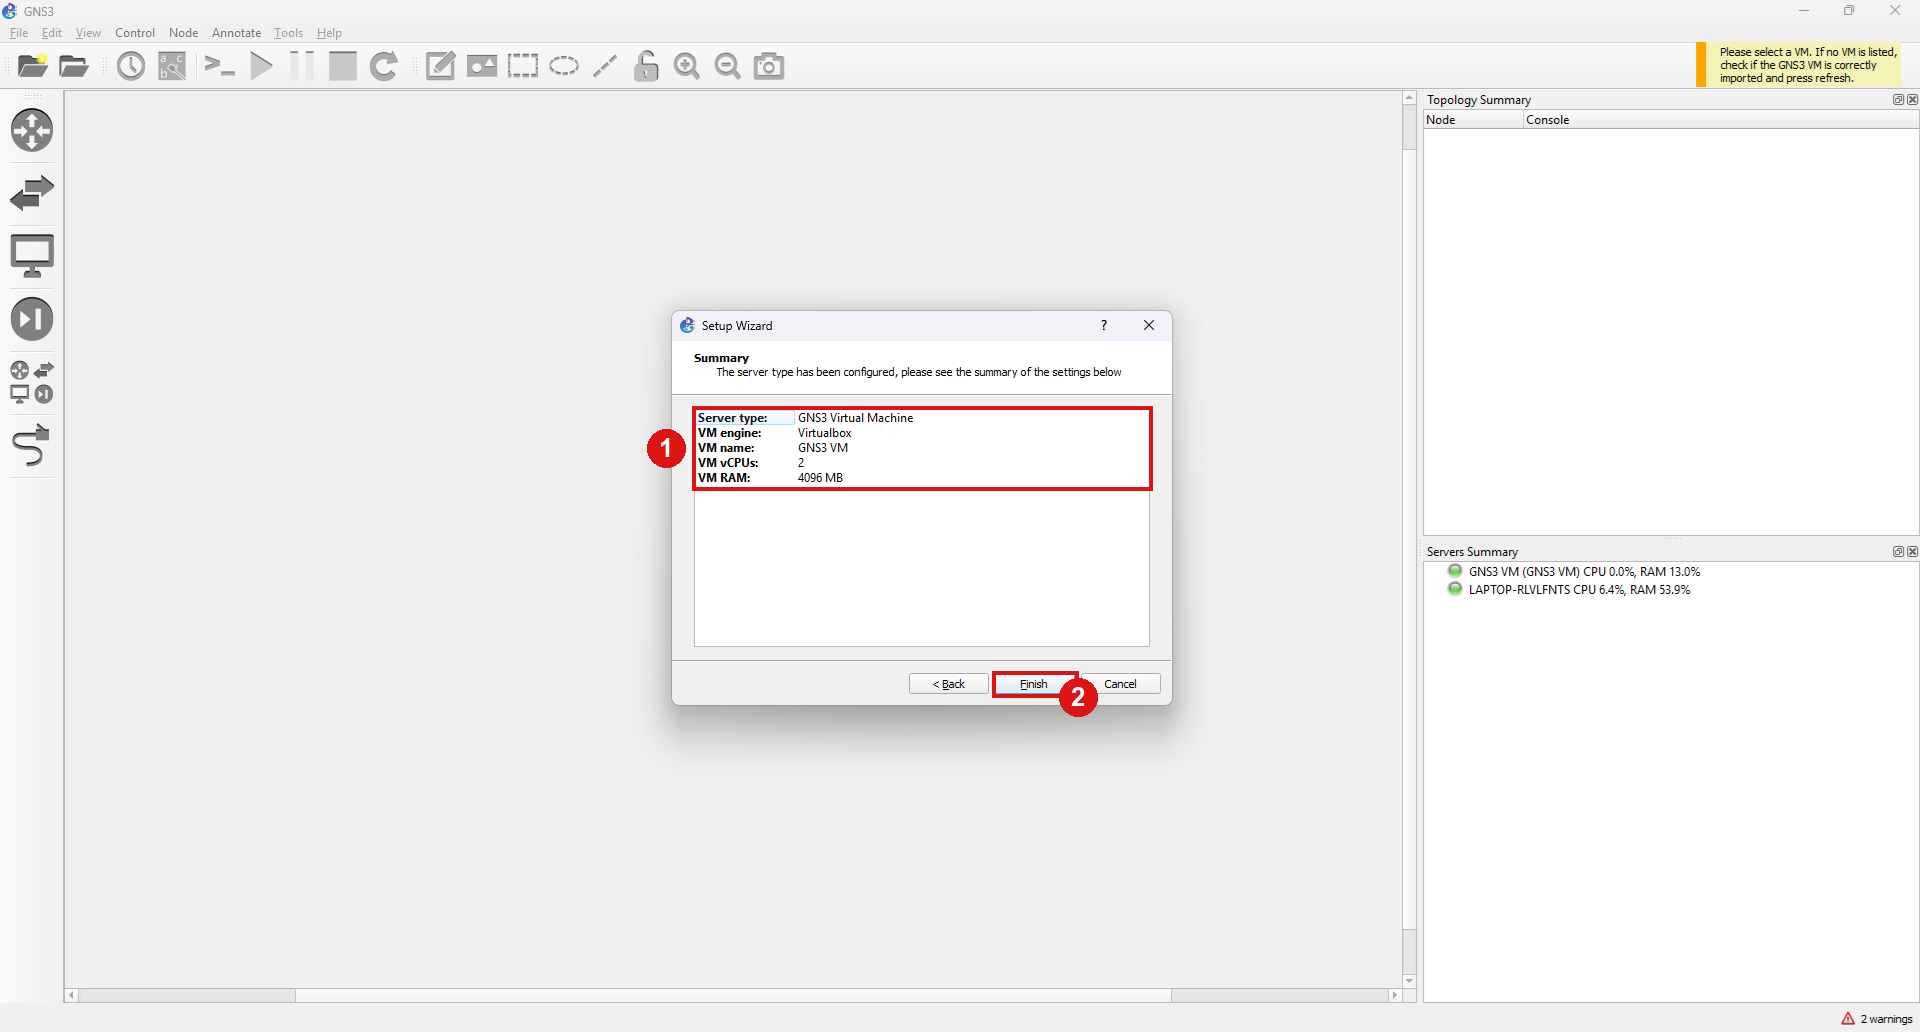
\includegraphics[width=\textwidth]{images/gns3_wizard_resumen.png}
    \caption{Asistente, paso 3: resumen de la configuración (1) y término del asistente (2).}
    \label{fig:wiz-resumen}
\end{figure}

Con GNS3 ya configurado, el siguiente paso es \textbf{crear un proyecto}, que es donde se construye la topología de red. Para ello abra el cuadro de diálogo \textit{Project} de cualquiera de estas dos formas (Figura~\ref{fig:nuevo-proyecto}):

\begin{itemize}
    \item Desde el menú \textbf{File} (1), opción \textit{New blank project}.
    \item Presionando el ícono de la \textbf{carpeta} ubicado bajo el menú \textit{File}, en la barra de herramientas (2).
\end{itemize}

En la pestaña \textit{New project} del cuadro que se abre, ingrese el nombre del proyecto y, si lo desea, su ubicación (3), y presione \textit{OK} (4). Desde este mismo cuadro, con \textit{Open a project from disk}, también se puede abrir un proyecto existente.

\begin{figure}[H]
    \centering
    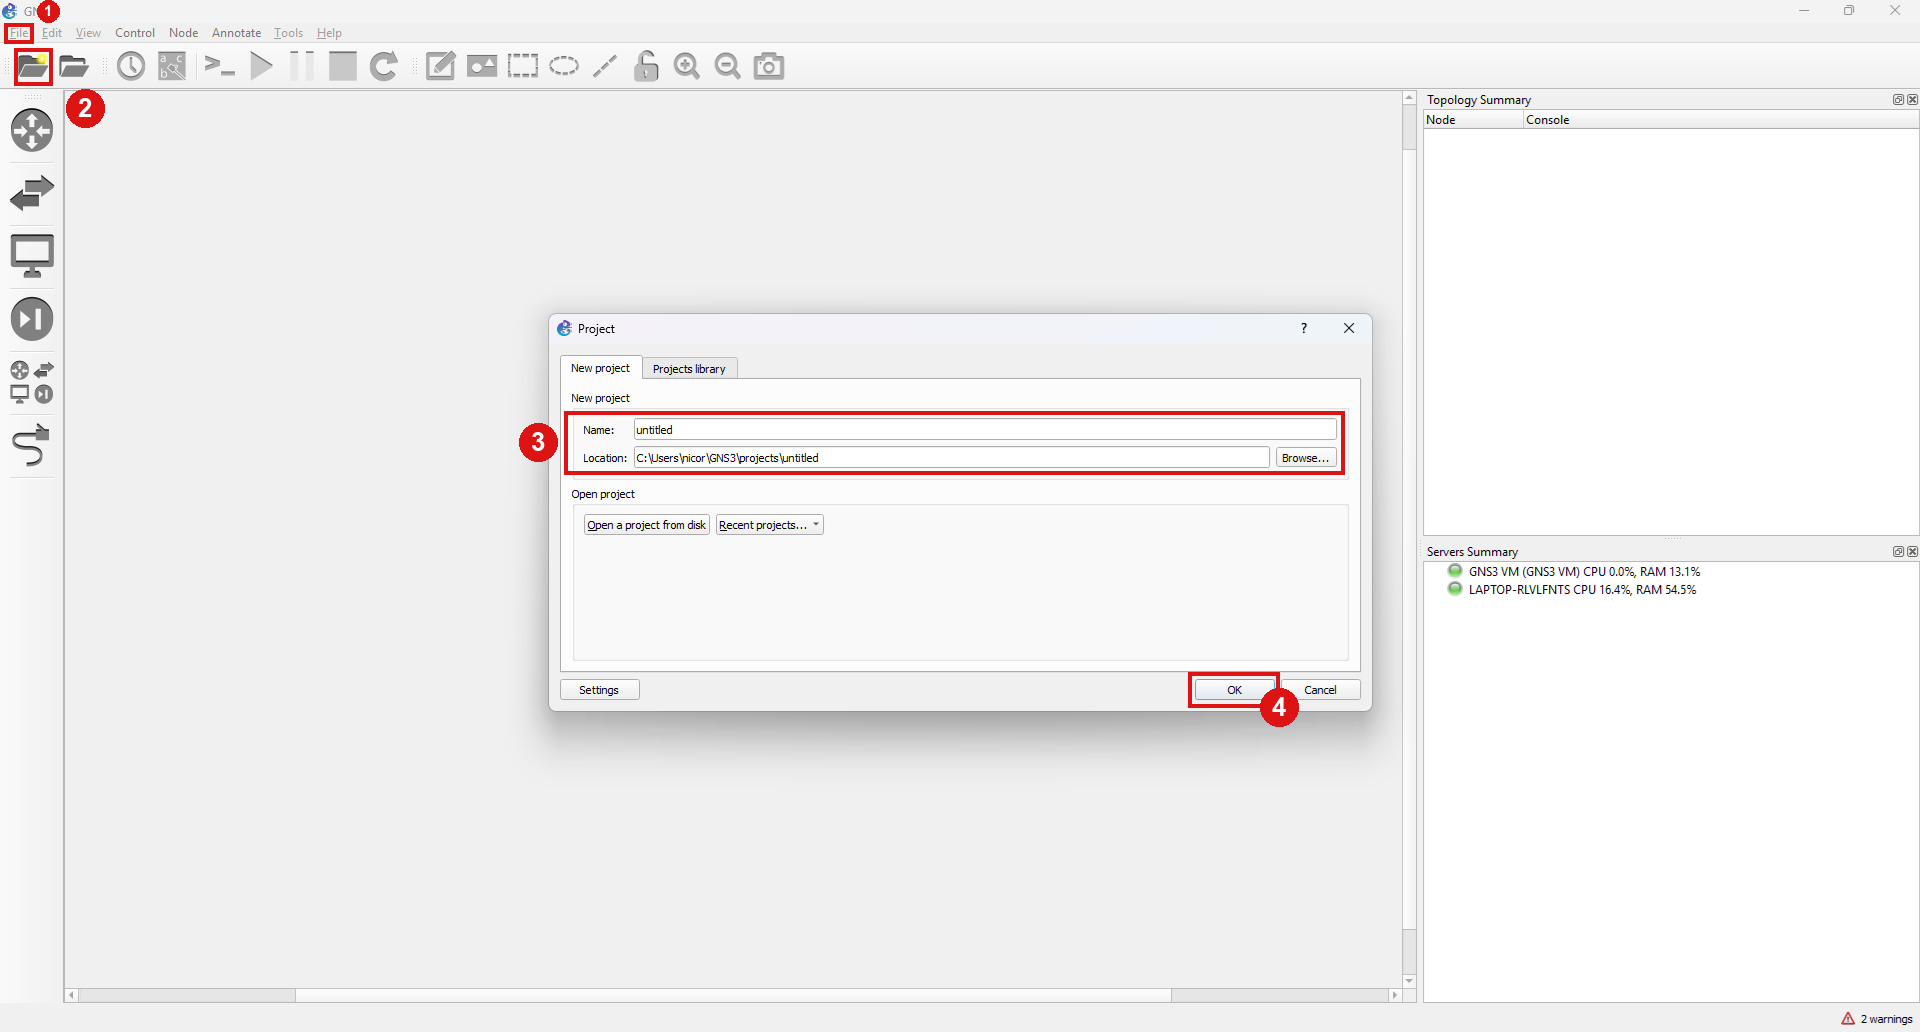
\includegraphics[width=\textwidth]{images/gns3_nuevo_proyecto.png}
    \caption{Creación de un proyecto nuevo: se abre desde el menú \textit{File} (1) o con el ícono de carpeta (2); luego se ingresan el nombre y la ubicación (3) y se confirma (4).}
    \label{fig:nuevo-proyecto}
\end{figure}

\subsection{Uso básico}

La Figura~\ref{fig:interfaz} muestra la ventana principal de GNS3 con un proyecto que contiene un router y dos VPCS. Sus partes principales son:

\begin{enumerate}
    \item \textbf{Barra de categorías de dispositivos}: cada ícono abre el ``cajón'' de una categoría: routers, switches, dispositivos terminales y dispositivos de seguridad. El último ícono (\textit{All devices}) muestra todos los dispositivos disponibles.
    \item \textbf{Agregar enlace} (\textit{Add a link}): activa la herramienta para conectar dispositivos con cables.
    \item \textbf{Cajón de dispositivos}: lista los dispositivos de la categoría seleccionada (en la figura, los routers). Con \textit{New template} se agregan dispositivos nuevos (ver \textit{Incorporación de componentes adicionales}).
    \item \textbf{Área de trabajo}: lienzo donde se construye la topología de red.
    \item \textbf{Controles de la simulación}: iniciar (triángulo verde), pausar (amarillo) y detener (rojo) todos los dispositivos del proyecto.
    \item \textbf{Paneles de resumen}: \textit{Topology Summary} lista los dispositivos del proyecto, su estado (verde encendido, rojo apagado) y la dirección de su consola; \textit{Servers Summary} muestra los servidores disponibles (la GNS3 VM y el computador local) y su uso de CPU y RAM.
\end{enumerate}

\begin{figure}[H]
    \centering
    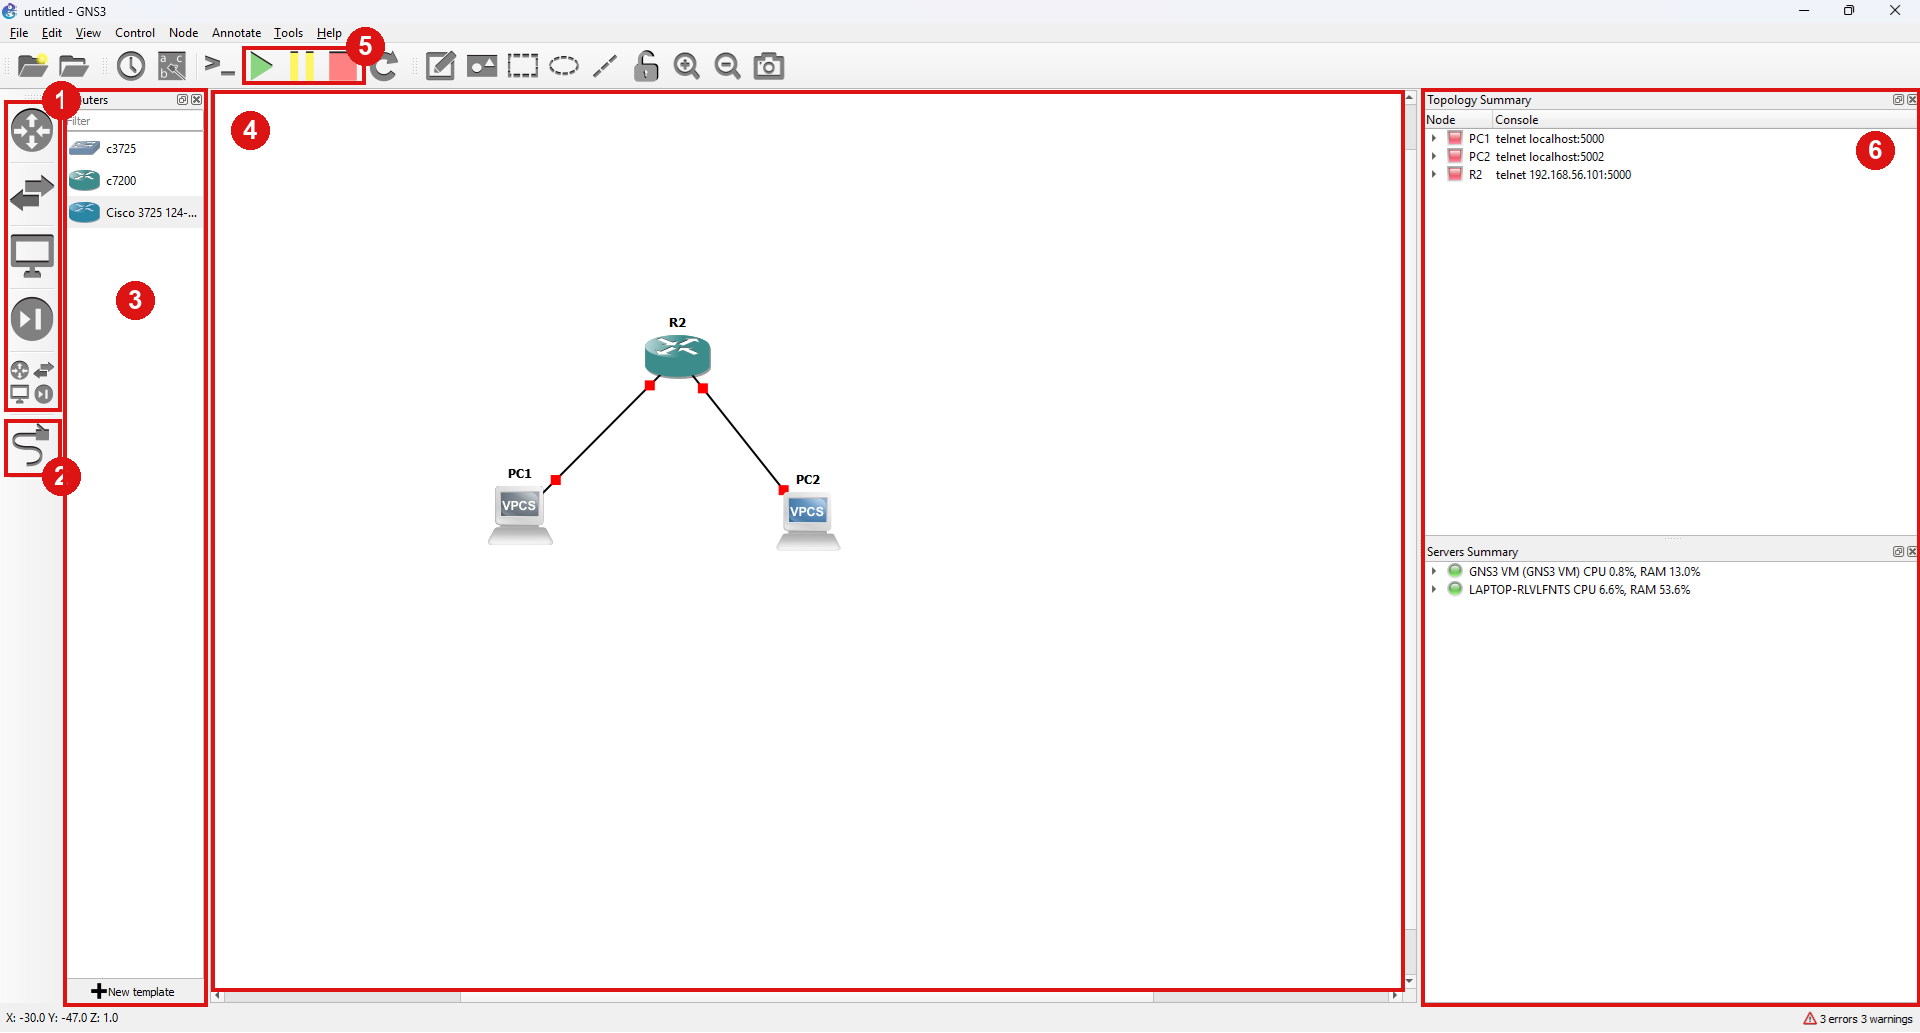
\includegraphics[width=\textwidth]{images/gns3_interfaz_principal.png}
    \caption{Ventana principal de GNS3: categorías de dispositivos (1), agregar enlace (2), cajón de dispositivos (3), área de trabajo (4), controles de la simulación (5) y paneles de resumen (6).}
    \label{fig:interfaz}
\end{figure}

Para agregar un dispositivo a la red, seleccione su categoría (1) y \textbf{arrástrelo desde el cajón (3) hasta el área de trabajo (4)}. Al soltarlo, si se trabaja con la GNS3 VM, puede aparecer una ventana preguntando si se desea ejecutar el dispositivo de forma local o en la máquina virtual. Luego se \textbf{conectan los dispositivos} activando la herramienta de agregar enlaces (2): haga clic en el primer dispositivo, elija la interfaz, y repita en el segundo dispositivo. Para comenzar la simulación se presiona el botón de inicio (5); también es posible iniciar o detener un dispositivo individual haciendo clic derecho sobre él. Para abrir la consola de un dispositivo encendido, haga doble clic sobre él.

\begin{nota}
Si modifica la configuración de un \textbf{template} (por ejemplo, la RAM o las opciones QEMU de una máquina), los nodos ya existentes en la topología \textbf{conservan la configuración antigua}. Debe \textbf{eliminarlos y volver a arrastrarlos} desde la barra lateral para que tomen la nueva configuración.
\end{nota}

\subsection{Exportar e Importar Proyectos}

GNS3 permite almacenar proyectos de simulación en un archivo comprimido único (extensión \texttt{.gns3project}), que además de la disposición de los equipos almacena sus configuraciones. Este archivo es el que se adjunta en la entrega de la tarea.

\begin{itemize}
    \item \textbf{Exportar:} con el proyecto abierto, vaya a \textit{File $>$ Export portable project}, elija la ubicación y el nombre del archivo y confirme. No es necesario incluir las imágenes base de los equipos (opción \textit{Include base images}), lo que mantiene el archivo liviano.
    \item \textbf{Importar:} vaya a \textit{File $>$ Import portable project}, seleccione el archivo \texttt{.gns3project} y asigne un nombre y ubicación al proyecto.
\end{itemize}

\subsection{Componentes}

Los componentes de interés para esta tarea son:

\begin{itemize}
    \item \textbf{Ethernet switch}: cumple las funcionalidades básicas de un switch (conmutación a nivel de capa de enlace).
    \item \textbf{VPCS}: simula un dispositivo terminal muy simple. Se le puede asignar una IP y realizar \texttt{ping}. Una vez corriendo, se abre su terminal con doble clic. Comandos útiles:
\end{itemize}

\begin{lstlisting}
ip 192.168.16.10 255.255.255.0 192.168.16.1   # IP, mascara y gateway
ip 10.1.1.17/26 10.1.1.1                       # forma abreviada
ip dhcp                                        # configurar por DHCP (respuesta DORA)
show ip                                        # mostrar configuracion IP
\end{lstlisting}

\begin{itemize}
    \item \textbf{Nube (Cloud)}: permite conectar la red a la red exterior por medio de una interfaz de red del equipo. Inicialmente no tiene ninguna interfaz configurada. Para agregarla, entre a \textit{Configure} (clic derecho sobre la nube) y añada la interfaz deseada.
\end{itemize}

\begin{nota}
Para la \textbf{Pregunta 3} (envío de video al PC personal) y la \textbf{Pregunta 4} se utiliza la nube conectada a una interfaz de la GNS3 VM en modo \textbf{bridge}. En VirtualBox, agregue a la GNS3 VM un \textbf{Adaptador puente (Bridged)} sobre su interfaz de red (idealmente por \textbf{cable Ethernet}). Dentro de la GNS3 VM ese adaptador aparece como \texttt{eth2}, que es la interfaz que debe seleccionar en la nube. Recuerde poner el \textbf{Modo Promiscuo} del adaptador en ``Permitir Todo''.
\end{nota}

\begin{nota}
Cuando se desea conectar las PC del entorno virtual de GNS3 con su PC real, es necesario \textbf{desactivar el firewall} (o el antivirus) del host para impedir que bloqueen la comunicación.
\end{nota}

\begin{nota}
\textbf{Limitación conocida del bridge sobre Wi-Fi:} el bridging de VirtualBox sobre una interfaz \textbf{inalámbrica} filtra las tramas cuyo origen es una MAC distinta a la del adaptador Wi-Fi. Esto impide que un router Cisco emulado (con su propia MAC) sea alcanzable desde un dispositivo externo (por ejemplo, un celular) a través del Wi-Fi. Para escenarios que requieran alcanzar equipos emulados desde fuera, use \textbf{conexión por cable Ethernet}.
\end{nota}

\subsubsection{Incorporación de componentes adicionales}

Para agregar componentes que no vienen incluidos en GNS3, descargue los archivos correspondientes (\textbf{Appliance} e \textbf{Imagen}, ver sección \textit{Recursos}). Luego use \textit{File $>$ Import Appliance}, seleccione el archivo \texttt{.gns3a} y siga el asistente. Al llegar a la pantalla de archivos requeridos, se listan las imágenes necesarias; si ya las descargó en la misma carpeta, deberían detectarse automáticamente. Si la versión no coincide, use \textit{Create a new version} e indique la ruta al archivo \texttt{.qcow2}.

Los componentes adicionales a utilizar son:

\begin{itemize}
    \item \textbf{NETem}: componente con dos interfaces de red que permite simular enlaces con características especiales (límites de ancho de banda, retardos y pérdidas). Una vez iniciado, se accede a su terminal de configuración con doble clic.
    \item \textbf{Máquina Alpine Linux}: máquina virtual liviana con todas las herramientas de la tarea preinstaladas (ver sección \textit{Máquina Virtual Alpine Linux}). Contraseña del usuario: \texttt{elo323}.
    \item \textbf{Router Cisco 3725}: posee dos interfaces FastEthernet para comunicar dos redes LAN. Para incorporarlo, despliegue \textit{Browse all devices $>$ +New template $>$ Import an appliance file} y escoja el appliance de ``Cisco 3725''. En el paso de versión, seleccione \textit{Create a new version} con el nombre \texttt{3725\_15.T}.
\end{itemize}

\begin{nota}
Para la \textbf{Pregunta 4}, el router Cisco 3725 requiere más recursos de los que trae por defecto. Antes de usarlo, aumente sus recursos en \textit{Edit $>$ Preferences $>$ IOS routers $>$ Cisco 3725 $>$ Edit $>$ Memories and disks}:
\begin{itemize}[leftmargin=1.2cm]
    \item \textbf{RAM: al menos 256 MB} (para soportar SIP/CME con dos teléfonos).
\end{itemize}
\end{nota}

\begin{nota}
Si al importar un componente no se detecta la imagen automáticamente, puede importarla manualmente con el botón \textit{Import}.
\end{nota}

\subsection{Ejecución sin KVM}

En equipos con \textbf{VirtualBox sobre Windows}, la virtualización anidada (KVM) suele no estar disponible. Sin KVM, las imágenes con kernels modernos pueden no arrancar (\textit{kernel panic: IO-APIC + timer doesn't work}). Para evitarlo:
\begin{itemize}[leftmargin=1.2cm]
    \item En el template QEMU (\textit{Edit $>$ Preferences $>$ QEMU VMs $>$ [máquina] $>$ Edit $>$ Advanced $>$ Options}) agregue: \texttt{-cpu qemu64}.
    \item La imagen Alpine provista ya está preparada para arrancar sin KVM.
\end{itemize}
El componente NETem también puede requerir \texttt{-cpu qemu64}. Sin KVM el rendimiento es menor; puede ser necesario reintentar el arranque de algún nodo.

\subsection{Captura de Paquetes}

Durante la instalación de GNS3 se ofrece instalar el capturador de paquetes \textbf{Wireshark}; el simulador permite capturar en cualquiera de los enlaces. Para ello, posicione el cursor sobre un enlace (se pondrá rojo), haga clic derecho y seleccione \textit{Iniciar Captura}. Basta con dejar el tipo de enlace en Ethernet. Al aceptar, se abrirá Wireshark con la captura.

\begin{nota}
\textbf{Para Linux:} si recibe un error indicando que \texttt{dumpcap} no tiene permisos, ejecute:
\begin{lstlisting}
cd /usr/bin/
sudo chmod +x dumpcap
\end{lstlisting}
\end{nota}

Para que Wireshark decodifique los paquetes RTP, habilite la opción \texttt{rtp\_udp} en el menú \textit{Analyze $>$ Enabled Protocols\ldots}

\subsection{Creación de VLAN en Ethernet Switch}

El switch Ethernet de GNS3 permite la creación de VLANs y puertos troncales de forma sencilla. Haga clic derecho sobre el switch y seleccione \textit{Configure}. Se abrirá una ventana con los puertos existentes; por defecto todos pertenecen a la VLAN 1. Para cambiar la VLAN de un puerto, seleccione el número y edítelo. En el campo \textit{Type} existen tres modos: \textit{access} (modo común, una sola VLAN por puerto), \textit{dot1q} (modo troncal, permite todas las VLANs) y \textit{qinq} (encapsulación IEEE 802.1ad o ``Q-in-Q'': agrega una segunda etiqueta VLAN sobre tramas que ya vienen etiquetadas, lo que permite, por ejemplo, que un proveedor transporte las VLANs de varios clientes por su red asignando una VLAN propia a cada cliente). Para almacenar los cambios, haga clic en \textit{Add}.

% ==================== ALPINE ====================
\section{Máquina Virtual Alpine Linux}

\subsection{¿Qué es Alpine Linux?}

\href{https://alpinelinux.org/}{Alpine Linux} es una distribución de Linux orientada a la seguridad, la simplicidad y la eficiencia de recursos. Está construida sobre \texttt{musl libc}\footnote{\texttt{musl} es una implementación liviana de la biblioteca estándar de C: \url{https://musl.libc.org/}} y BusyBox\footnote{BusyBox reúne en un único ejecutable versiones reducidas de las utilidades de Unix más comunes (\texttt{ls}, \texttt{cp}, \texttt{sh}, etc.): \url{https://busybox.net/}}, lo que la hace extremadamente compacta. Es muy utilizada en contenedores (Docker) y en entornos donde el tamaño y la velocidad de arranque son críticos. Sus principales ventajas para esta tarea son:

\begin{itemize}
    \item \textbf{Muy liviana}: la imagen completa pesa $\sim$595 MB.
    \item \textbf{Arranque rápido}: inicia en pocos segundos, incluso sin KVM.
    \item \textbf{Bajo consumo de RAM}: funciona con 512 MB.
    \item \textbf{Sin entorno gráfico}: se opera por terminal, lo que es más representativo de servidores reales y refuerza el manejo de línea de comandos.
\end{itemize}

\subsection{Credenciales y contenido}

\begin{center}
\begin{tabular}{|l|l|}
    \hline
    \textbf{Usuario administrador} & \texttt{root} / \texttt{elo323} \\ \hline
    \textbf{Usuario normal}        & \texttt{elo323} / \texttt{elo323} \\ \hline
\end{tabular}
\end{center}

\begin{nota}
El usuario \texttt{elo323} se usa para ejecutar VLC, ya que \textbf{VLC no se ejecuta como root}. Para tareas de captura (\texttt{tcpdump}, \texttt{tshark}) se requieren privilegios de \texttt{root} (use \texttt{su -}).
\end{nota}

La imagen trae preinstaladas las siguientes herramientas: \texttt{iperf} e \texttt{iperf3} (Pregunta 2), \texttt{vlc}/\texttt{cvlc} (Pregunta 3), \texttt{tcpdump} y \texttt{tshark} (captura y análisis), \texttt{pjsua} (Pregunta 4), además de \texttt{sox}, \texttt{ffmpeg}, \texttt{curl} y \texttt{openssh}. Incluye también los siguientes archivos multimedia:

\begin{itemize}
    \item \texttt{/home/elo323/Videos/sample.mp4}: video para la Pregunta 3.
    \item \texttt{/home/elo323/test\_audio.wav}: audio de voz en español para la Pregunta 4.
\end{itemize}

\subsection{Configuración de red manual}

La imagen no configura IP automáticamente; se asigna de forma manual. Ejemplo:

\begin{lstlisting}
ip addr flush dev eth0
ip addr add 192.168.4.10/24 dev eth0
ip link set eth0 up
ip route add default via 192.168.4.1
ping 192.168.4.1 -c 3
\end{lstlisting}

\begin{nota}
Apague siempre la máquina de forma limpia con el comando \texttt{poweroff} desde su consola. Detenerla forzadamente (Stop) puede corromper su sistema de archivos.
\end{nota}

\subsection{Importación de la imagen en GNS3}

Cree un nuevo template QEMU en \textit{Edit $>$ Preferences $>$ QEMU VMs $>$ New} con estos parámetros:

\begin{center}
\begin{tabular}{|l|l|}
    \hline
    Nombre            & \texttt{Alpine-ELO323} \\ \hline
    Qemu binary       & \texttt{/bin/qemu-system-x86\_64} \\ \hline
    RAM               & 512 MB \\ \hline
    Console type      & \texttt{telnet} \\ \hline
    Disk image (hda)  & \texttt{alpine-elo323.qcow2} \\ \hline
    Advanced $>$ Options & \texttt{-cpu qemu64} \\ \hline
\end{tabular}
\end{center}

\begin{nota}
La opción \texttt{-cpu qemu64} es obligatoria si no se dispone de KVM (ver sección \textit{Ejecución sin KVM}).
\end{nota}

% ==================== STREAMING VLC ====================
\section{Streaming con VLC}

En la máquina Alpine, VLC se ejecuta en modo consola con el comando \texttt{cvlc} (VLC sin interfaz gráfica), bajo el usuario \texttt{elo323}. Permite emitir y recibir flujos de video mediante RTP.

\subsection{RTP}

En Alpine, VLC se utiliza desde la línea de comandos. Cambie primero al usuario \texttt{elo323}:
\begin{lstlisting}
su - elo323
\end{lstlisting}

Para \textbf{transmitir} el video por RTP hacia una IP destino (unicast) o de broadcast:

\begin{lstlisting}
cvlc /home/elo323/Videos/sample.mp4 --loop \
     --sout '#rtp{dst=IP_DESTINO,port=5004,mux=ts}' --sout-keep
\end{lstlisting}

Para \textbf{recibir} el flujo en el equipo destino (por ejemplo, su PC personal en la Pregunta 3.c) se necesita un reproductor capaz de abrir un flujo RTP. Dos opciones compatibles, disponibles para Windows, Linux y macOS:

\begin{itemize}
    \item \textbf{VLC media player} (\href{https://www.videolan.org/vlc/}{videolan.org}): abra \textit{Medio $>$ Abrir ubicación de red} (\textit{Media $>$ Open Network Stream} en inglés, atajo \texttt{Ctrl+N}), ingrese la URL \texttt{rtp://@:5004} y presione \textit{Reproducir}. El símbolo \texttt{@} indica que se escuchan los paquetes que llegan al puerto 5004 en cualquier interfaz del equipo. Equivalentemente, desde una terminal:
\begin{lstlisting}
vlc rtp://@:5004
\end{lstlisting}
    \item \textbf{ffplay}, reproductor incluido en \href{https://ffmpeg.org/download.html}{FFmpeg}: desde una terminal ejecute
\begin{lstlisting}
ffplay rtp://0.0.0.0:5004
\end{lstlisting}
    donde \texttt{0.0.0.0} indica, igual que \texttt{@} en VLC, que se escucha en todas las interfaces.
\end{itemize}

No es necesario que la transmisión haya comenzado antes de abrir el flujo en el receptor; el reproductor comenzará a mostrar el video automáticamente al recibir datos. Recuerde que el firewall del equipo receptor debe permitir el tráfico UDP entrante en el puerto 5004.

\begin{nota}
Para que Wireshark decodifique los paquetes RTP, habilite \texttt{rtp\_udp} en \textit{Analyze $>$ Enabled Protocols\ldots}
\end{nota}

\subsection{RTSP}

Para transmitir por RTSP, VLC actúa como servidor y el receptor solicita el flujo con una URL del tipo \texttt{rtsp://ip\_fuente:puerto/filename}. Los pasos son análogos a RTP.

\begin{investigar}
La construcción del comando \texttt{cvlc} para transmitir por \textbf{RTSP} (en lugar de RTP), así como el ajuste del \textit{caching} de red del receptor para observar el efecto del buffer, se dejan como investigación del estudiante. Revise la documentación de VLC sobre la opción \texttt{--sout} y el módulo \texttt{rtsp}.
\end{investigar}

% ==================== IPERF ====================
\section{iperf}

\texttt{iperf} es un programa de línea de comando que permite medir el ancho de banda entre dos equipos, disponible en la máquina Alpine. Funciona con un modelo cliente-servidor. En el servidor:

\begin{lstlisting}
iperf -s
\end{lstlisting}

En el cliente:

\begin{lstlisting}
iperf -c <direccion_ip_del_servidor>
\end{lstlisting}

Es posible configurar el tiempo de prueba con la opción \texttt{-t}. Al terminar, los resultados se imprimen en ambas terminales.

\begin{nota}
\texttt{iperf} usa una conexión \textbf{TCP} por defecto para medir ancho de banda. La imagen incluye también \texttt{iperf3}.
\end{nota}

\begin{investigar}
La medición con \textbf{UDP} (opción \texttt{-u}) y la interpretación de la diferencia entre el throughput TCP y UDP sobre un enlace con pérdidas se dejan como investigación del estudiante.
\end{investigar}

% ==================== VOIP ====================
\section{Telefonía VoIP con SIP}

Esta sección cubre la configuración del \textbf{servidor SIP (Call Manager Express, CME) integrado al router Cisco 3725} y el uso del softphone de consola \texttt{pjsua} en la máquina Alpine, para las preguntas 4.a y 4.b.

\subsection{Conceptos generales}

En una llamada VoIP con SIP intervienen dos planos: la \textbf{señalización SIP} (mensajes \texttt{REGISTER}, \texttt{INVITE}, \texttt{ACK}, \texttt{BYE}, etc., que establecen y terminan la llamada) y el \textbf{flujo de medios RTP} (los paquetes de audio propiamente tales). Además de las funciones normales de un router, el modelo Cisco 3725 incluye un servidor SIP (CME), que en esta tarea es el \textbf{registrar/servidor SIP}: los softphones se registran en él con un número de extensión y una contraseña, y a través de él se establecen las llamadas.

\subsection{Preparación del router Cisco 3725}

\begin{nota}
Recuerde aumentar la \textbf{RAM del router a 256 MB} antes de configurar su servidor SIP (ver sección \textit{Incorporación de componentes adicionales}). Con la RAM por defecto (128 MB) el servicio SIP/CME puede fallar por falta de memoria.
\end{nota}

Configure primero las interfaces de red del router según la topología. Por ejemplo, para dos redes internas:

\begin{lstlisting}
enable
configure terminal
interface fa0/0
 ip address 192.168.10.1 255.255.255.0
 no shutdown
 exit
interface fa0/1
 ip address 192.168.4.1 255.255.255.0
 no shutdown
 exit
\end{lstlisting}

\subsection{Configuración del servidor SIP (CME)}

La configuración base del servicio de voz y del registrar SIP es la siguiente:

\begin{lstlisting}
voice service voip
 allow-connections sip to sip
 sip
  registrar server expires max 3600
  exit
 exit

voice register global
 mode cme
 source-address 192.168.10.1 port 5060
 max-dn 10
 max-pool 10
 authenticate register
 exit
\end{lstlisting}

Luego se definen las extensiones (Directory Numbers) y los ``pools'' que asocian cada extensión a un usuario/contraseña SIP:

\begin{lstlisting}
voice register dn 1
 number 1001
 exit
voice register dn 2
 number 1002
 exit

voice register pool 1
 id mac 0000.0000.0001
 number 1 dn 1
 codec g711ulaw
 username 1001 password elo323
 exit
voice register pool 2
 id mac 0000.0000.0002
 number 1 dn 2
 codec g711ulaw
 username 1002 password elo323
 exit
\end{lstlisting}

Guarde la configuración con \texttt{end} y luego \texttt{write memory}. Puede verificar el estado del servidor SIP y de los registros con:

\begin{lstlisting}
show sip-ua status
show voice register global
show voice register pool all
\end{lstlisting}

\begin{investigar}
El escenario de la \textbf{Pregunta 4.b} requiere que la señalización SIP y el flujo RTP salgan por una interfaz específica del router (por ejemplo, cuando existe NAT o distintas subredes). Los comandos \texttt{bind control source-interface} y \texttt{bind media source-interface} (dentro de \texttt{voice service voip $>$ sip}) controlan este comportamiento, y el manejo de NAT para SIP/RTP (\texttt{ip nat service sip}) es un tema no trivial. Se deja como \textbf{investigación del estudiante} determinar la configuración necesaria según la topología escogida.
\end{investigar}

\subsection{Softphone pjsua}

Este año usted usará \texttt{pjsua}, un cliente SIP de línea de comandos (parte de la librería PJSIP) incluido en la imagen Alpine. Implementa el estándar SIP (RFC 3261), por lo que la señalización observable en la red es equivalente a la de un softphone comercial.

Para \textbf{registrar} un softphone en el servidor SIP del Cisco 3725 y dejarlo a la espera de llamadas (contestando automáticamente y grabando el audio recibido):

\begin{lstlisting}
pjsua --id="sip:1002@192.168.10.1" \
      --registrar="sip:192.168.10.1:5060" \
      --realm="*" \
      --username="1002" \
      --password="elo323" \
      --null-audio \
      --auto-answer=200 \
      --auto-rec \
      --rec-file=/home/elo323/audio_recibido.wav \
      --add-codec pcmu --clock-rate 8000
\end{lstlisting}

Para el softphone que \textbf{origina} la llamada y reproduce un archivo de audio como fuente:

\begin{lstlisting}
pjsua --id="sip:1001@192.168.10.1" \
      --registrar="sip:192.168.10.1:5060" \
      --realm="*" \
      --username="1001" \
      --password="elo323" \
      --null-audio \
      --play-file=/home/elo323/test_audio.wav --auto-play \
      --add-codec pcmu --clock-rate 8000
\end{lstlisting}

Una vez registrado (debe aparecer \texttt{registration success, status=200 (OK)}), dentro de la consola interactiva de \texttt{pjsua} se realiza la llamada con la tecla \texttt{m} e ingresando la URI destino, por ejemplo \texttt{sip:1002@192.168.10.1}. Para colgar se usa \texttt{h} y para salir \texttt{q}.

\begin{nota}
Las opciones \texttt{--null-audio} (evita usar tarjeta de sonido, que no existe en Alpine), \texttt{--add-codec pcmu} y \texttt{--clock-rate 8000} fuerzan el uso de \textbf{G.711 $\mu$-law a 8000 Hz}, el códec estándar de la tarea.
\end{nota}

\subsection{Análisis de la señalización y el audio}

Durante la llamada puede capturar la señalización SIP y el flujo RTP con \texttt{tcpdump} (como \texttt{root}) y analizarlos con \texttt{tshark}:

\begin{lstlisting}
tcpdump -i eth0 -w /tmp/voip.pcap -c 300
tshark -r /tmp/voip.pcap -Y "sip" -T fields -e sip.Method -e sip.Status-Code
\end{lstlisting}

\begin{investigar}
El análisis de la \textbf{periodicidad de los paquetes RTP}, la identificación del \textbf{códec negociado} en el intercambio SDP y la interpretación de la secuencia completa de mensajes SIP (\texttt{REGISTER} 401/200, \texttt{INVITE} 100/200, \texttt{ACK}, \texttt{BYE}) se dejan como investigación del estudiante a partir de las capturas obtenidas.
\end{investigar}

\subsection{Extracción de las grabaciones de audio}

Para analizar el audio recibido (Pregunta 4.b), las grabaciones \texttt{.wav} generadas dentro de la máquina Alpine deben copiarse al computador personal. Consulte la sección \textit{QEMU -- Montar imágenes} para el procedimiento de montaje del disco de la máquina y extracción de los archivos.

% ==================== QEMU ====================
\section{QEMU (Quick EMUlator)}

QEMU es un emulador de sistemas que permite correr máquinas virtuales de equipos con diferentes arquitecturas. Gracias a esto, GNS3 puede simular una gran variedad de hardware de red.

\subsection{Crear una máquina virtual}

Las máquinas virtuales de la tarea corren sobre esta plataforma y ya están listas para su uso, pero puede ser de interés crear una propia. Se crea una imagen de disco con \texttt{qemu-img}:

\begin{lstlisting}
qemu-img create -f qcow2 imagen.qcow2 10G
\end{lstlisting}

La opción \texttt{-f} indica el formato; \texttt{qcow2} crea una imagen que crece a medida que se escribe el disco. Para ejecutarla e instalar un sistema operativo desde una ISO:

\begin{lstlisting}
qemu-system-x86_64 -hda imagen.qcow2 -cdrom <imagen_so> -boot d
\end{lstlisting}

Para ejecutar una imagen ya instalada asignándole memoria:

\begin{lstlisting}
qemu-system-x86_64 -hda imagen.qcow2 -boot c -m <memoria>
\end{lstlisting}

\begin{nota}
Si ejecuta una máquina sin KVM disponible, agregue la opción \texttt{-cpu qemu64}:
\begin{lstlisting}
qemu-system-x86_64 -cpu qemu64 -m 512 -hda imagen.qcow2 -nographic
\end{lstlisting}
\end{nota}

\subsection{Montar imágenes}

Para transferir archivos desde una máquina virtual de QEMU (por ejemplo, extraer las grabaciones de audio de la Pregunta 4.b), es posible montar su imagen en el sistema de archivos del host:

\begin{lstlisting}
sudo modprobe nbd max_part=8
sudo qemu-nbd --connect=/dev/nbd0 [ruta_a_la_imagen.qcow2]
sudo mount /dev/nbd0p3 /mnt
\end{lstlisting}

Esto activa el módulo \texttt{nbd}, conecta la imagen como dispositivo \texttt{nbd0} y monta su partición. Las imágenes de los equipos usados en GNS3 se encuentran en \texttt{project-files/qemu} dentro de la carpeta del proyecto.

\begin{nota}
En la imagen Alpine, el sistema de archivos raíz está en la \textbf{partición 3} (\texttt{/dev/nbd0p3}), por lo que se monta esa partición (en otras imágenes puede ser \texttt{p1}). Los archivos del usuario están en \texttt{/home/elo323/}.
\end{nota}

Una vez terminado el trabajo con la imagen, desmóntela:

\begin{lstlisting}
sudo umount /mnt
sudo qemu-nbd --disconnect /dev/nbd0
sudo modprobe -r nbd
\end{lstlisting}

\begin{nota}
Realice el montaje únicamente con la máquina \textbf{apagada} en GNS3; de lo contrario el disco estará en uso y el montaje fallará o corromperá datos. Tenga cuidado de no montar la imagen base mientras un nodo la esté usando.
\end{nota}

% ==================== RECURSOS ====================
\section{Recursos}

\subsection{Appliances e imágenes de GNS3}

\begin{center}
\renewcommand{\arraystretch}{1.3}
\begin{tabularx}{\textwidth}{|l|X|l|}
    \hline
    \textbf{Recurso} & \textbf{Fuente} & \textbf{Tamaño} \\ \hline
    Appliance NETem & \href{https://www.gns3.com/marketplace/appliance/netem}{Link} & 1.7 K \\ \hline
    Imagen NETem & \href{https://github.com/phobozad/NETem/releases/download/v4.1/NETem-v4.1.qcow2}{Link} & 25 M \\ \hline
    Imagen Alpine ELO323 & \href{https://profesores.elo.utfsm.cl/\string~agv/elo323.ipd438/2s26/Assignment/alpine-elo323-entrega.qcow2.gz}{Link} & $\sim$595 M \\ \hline
    Appliance Cisco 3725 & \href{https://gns3.com/marketplace/appliances/cisco-3725}{Link} & 1.1 K \\ \hline
    Imagen Cisco 3725 & \href{https://archive.org/download/c2691-adventerprisek9-mz.124-15.T14/c3725-adventerprisek9-mz.124-15.T14.bin}{Link} & 44 M \\ \hline
\end{tabularx}
\end{center}

La imagen \texttt{alpine-elo323.qcow2} se distribuye comprimida a través del servidor del curso: \\
\url{https://profesores.elo.utfsm.cl/~agv/elo323.ipd438/2s26/Assignment/alpine-elo323-entrega.qcow2.gz}

Antes de importarla en GNS3, descomprima el archivo \texttt{.gz} (por ejemplo, con 7-Zip en Windows o con \texttt{gunzip} en Linux).

% ==================== CRÉDITOS ====================
\section{Créditos}

\begin{itemize}[leftmargin=1.2cm]
    \item \textbf{Revisión 2\textordmasculine{} Semestre 2026 por Nicolás Rogel}
    \item Revisión 2\textordmasculine{} Semestre 2025 por Sebastián Madariaga
    \item Revisión 2\textordmasculine{} Semestre 2024 por Carlos Soto
    \item Revisión 2\textordmasculine{} Semestre 2023 por Sebastián Castillo
    \item Revisión 2\textordmasculine{} Semestre 2022 por Nicolás Miranda
    \item Revisión 2\textordmasculine{} Semestre 2020--21 por Loreto Romero
    \item Revisión 2\textordmasculine{} Semestre 2019 por Dayana Hernández
    \item Revisión 2\textordmasculine{} Semestre 2018 por Jesús Márquez
    \item Revisión 2\textordmasculine{} Semestre 2017 por Hans Lehnert
\end{itemize}

\end{document}
